% !TeX program = lualatex
% !BIB program = bibtex
\documentclass[a4paper,12pt,twoside,openany]{report}

\newcommand{\autorpracy}{Jakub Mikusek}
\newcommand{\numeralbumu}{160776}
\newcommand{\tytulpl}{Metoda oceny mechanizmu Data Availability Sampling w modularnych warstwach dostępności danych w systemach blockchain}
\newcommand{\tytulen}{ A Method for Evaluating Data Availability Sampling in Modular Data Availability Layers of Blockchain Systems}
\newcommand{\rodzajpracy}{magisterska}
\newcommand{\kierunek}{Informatyka}
\newcommand{\specjalnosc}{Cyberbezpieczeństwo}
\newcommand{\promotor}{dr inż. Andrzej Wilczyński}
\newcommand{\miejsce}{Kraków}
\newcommand{\rokpracy}{2027}

\usepackage{iftex}
\RequireLuaTeX
\usepackage[polish]{babel}
\usepackage{amsmath}
\usepackage{fontspec}
\usepackage{unicode-math}

\IfFontExistsTF{Times New Roman}
  {\setmainfont{Times New Roman}}
  {\setmainfont{TeX Gyre Termes}}
\setmathfont{TeX Gyre Termes Math}
\IfFontExistsTF{Arial}
  {\newfontfamily\fonttytulowa{Arial}}
  {\newfontfamily\fonttytulowa{TeX Gyre Heros}}

\usepackage{luavlna}
\singlechars{polish}{AaIiOoUuWwZz}

\usepackage{microtype}

\usepackage[a4paper, twoside,
            top=2.5cm, bottom=2.5cm, inner=3.5cm, outer=2.5cm,
            headheight=0pt, headsep=0pt, footskip=1.25cm]{geometry}

\usepackage{setspace}
\setstretch{1.43}

\setlength{\parindent}{1.25cm}
\setlength{\parskip}{0pt}
\usepackage{indentfirst}
\setlength{\emergencystretch}{2em}
\widowpenalty=10000
\clubpenalty=10000

\usepackage{fancyhdr}
\fancypagestyle{plain}{%
  \fancyhf{}%
  \fancyfoot[C]{\fontsize{10pt}{12pt}\selectfont\thepage}%
  \renewcommand{\headrulewidth}{0pt}%
  \renewcommand{\footrulewidth}{0pt}%
}
\pagestyle{plain}

\usepackage{titlesec}
\newcommand{\fontnaglowkaI}{\normalfont\fontsize{12pt}{14.5pt}\selectfont\bfseries}
\titleformat{\chapter}[block]{\fontnaglowkaI}{\thechapter.}{0.5em}{\MakeUppercase}
\titleformat{name=\chapter,numberless}[block]{\fontnaglowkaI}{}{0pt}{\MakeUppercase}
\titlespacing{\chapter}{0pt}{12pt}{6pt}
\titleformat{\section}{\normalfont\fontsize{10pt}{12pt}\selectfont\bfseries\itshape}{\thesection.}{0.5em}{}
\titlespacing{\section}{0pt}{12pt}{6pt}
\titleformat{\subsection}{\normalfont\fontsize{10pt}{12pt}\selectfont\itshape}{\thesubsection.}{0.5em}{}
\titlespacing{\subsection}{0pt}{12pt}{6pt}
\setcounter{secnumdepth}{2}
\setcounter{tocdepth}{2}

\usepackage[titles]{tocloft}
\renewcommand{\cftchapfont}{\normalfont}
\renewcommand{\cftchappagefont}{\normalfont}
\renewcommand{\cftchapleader}{\cftdotfill{\cftdotsep}}
\renewcommand{\cftchapaftersnum}{.}
\renewcommand{\cftsecaftersnum}{.}
\renewcommand{\cftsubsecaftersnum}{.}
\renewcommand{\cftfigaftersnum}{.}
\renewcommand{\cfttabaftersnum}{.}
\setlength{\cftbeforechapskip}{6pt}
\setlength{\cftbeforesecskip}{6pt}
\setlength{\cftbeforesubsecskip}{6pt}
\setlength{\cftbeforefigskip}{6pt}
\setlength{\cftbeforetabskip}{6pt}
\setlength{\cftchapnumwidth}{1.6em}
\setlength{\cftsecindent}{1.6em}
\setlength{\cftsecnumwidth}{2.6em}
\setlength{\cftsubsecindent}{4.2em}
\setlength{\cftsubsecnumwidth}{3.4em}
\setlength{\cftfigindent}{0pt}
\setlength{\cftfignumwidth}{2.8em}
\setlength{\cfttabindent}{0pt}
\setlength{\cfttabnumwidth}{2.8em}

\usepackage{graphicx}
\usepackage{array}
\usepackage{tabularx}
\usepackage{longtable}
\usepackage{multirow}
\usepackage{booktabs}
\usepackage{etoolbox}
\usepackage{caption}
\DeclareCaptionFont{dziesiec}{\linespread{1}\fontsize{10pt}{12pt}\selectfont}
\captionsetup{font=dziesiec, labelsep=period}
\captionsetup[table]{name=Tabela, position=above, labelfont=bf,
                     justification=raggedright, singlelinecheck=false, skip=4pt}
\captionsetup[figure]{name=Rys., position=below, justification=centering, skip=6pt}
\makeatletter
\let\pk@xfloat\@xfloat
\def\@xfloat#1[#2]{%
  \pk@xfloat#1[#2]%
  \ifdefstring{\@captype}{table}{\fontsize{10pt}{12pt}\selectfont}{}%
  \ifdefstring{\@captype}{figure}{\centering}{}}
\makeatother
\AtBeginEnvironment{longtable}{\fontsize{10pt}{12pt}\selectfont}
\renewcommand{\arraystretch}{1.2}
\setlength{\intextsep}{12pt plus 2pt minus 2pt}
\setlength{\textfloatsep}{12pt plus 2pt minus 2pt}
\setlength{\floatsep}{12pt plus 2pt minus 2pt}

\usepackage{tikz}
\usetikzlibrary{calc, positioning, arrows.meta}

\usepackage{listings}
\lstset{
  basicstyle=\ttfamily\fontsize{9pt}{11pt}\selectfont,
  columns=fullflexible, keepspaces=true,
  breaklines=true, showstringspaces=false,
  frame=single, numbers=left, numberstyle=\tiny, numbersep=6pt,
  captionpos=t, aboveskip=12pt, belowskip=12pt,
}
\renewcommand{\lstlistingname}{Listing}
\renewcommand{\lstlistlistingname}{Spis listingów}
\captionsetup[lstlisting]{labelfont=bf, justification=raggedright, singlelinecheck=false, skip=4pt}
\makeatletter
\renewcommand*{\l@lstlisting}[2]{%
  \vskip 6pt
  \begingroup
    \let\pk@numberline\numberline
    \def\numberline##1{\pk@numberline{##1.}}%
    \@dottedtocline{1}{0pt}{2.8em}{#1}{#2}%
  \endgroup}
\makeatother

\usepackage{enumitem}
\setlist{nosep}
\setlist[itemize,1]{label=\textbullet, leftmargin=1.27cm}
\setlist[enumerate,1]{label=\arabic*., leftmargin=1.27cm}

\newcommand{\wektor}[1]{\symbf{#1}}
\newcommand{\macierz}[1]{\symbf{#1}}

\usepackage{cite}
\makeatletter
\renewcommand{\@biblabel}[1]{#1.}
\makeatother
\apptocmd{\thebibliography}{\setlength{\itemsep}{6pt}\setlength{\parsep}{0pt}}{}{}

\usepackage{xurl}
\urlstyle{same}
\usepackage[hidelinks]{hyperref}
\hypersetup{
  pdftitle={\tytulpl},
  pdfauthor={\autorpracy},
  pdflang={pl-PL},
}
\usepackage{bookmark}

\newcommand{\rozdzialnienumerowany}[1]{%
  \chapter*{#1}%
  \phantomsection
  \addcontentsline{toc}{chapter}{#1}%
}

\newcommand{\spiswtresci}[2]{%
  \clearpage
  \phantomsection
  \addcontentsline{toc}{chapter}{#1}%
  \begin{singlespace}#2\end{singlespace}%
}

\makeatletter
\newcommand{\pk@blokmin}[2]{%
  \setbox\z@\vtop{\hsize=\linewidth\centering #2\par}%
  \ifdim\dimexpr\ht\z@+\dp\z@\relax<#1\relax
    \vtop to #1{\unvbox\z@\vfil}%
  \else
    \box\z@\par\vskip 0.4cm%
  \fi}
\newcommand{\stronatytulowa}{%
  \thispagestyle{empty}%
  \begingroup
  \setstretch{1}%
  \fonttytulowa
  \noindent
  \begin{tikzpicture}[remember picture, overlay,
      every node/.style={inner sep=0pt, outer sep=0pt}]
    \coordinate (M) at ($(current page.north west)+(2.5cm,-2.5cm)$);
    \node[anchor=north west] at ($(M)+(0.1cm,0)$)
      {
\includegraphics[width=2.16cm,height=2.31cm]{grafika/logo-pk.png}};
    \node[anchor=north east] at ($(M)+(15.8cm,0)$)
      {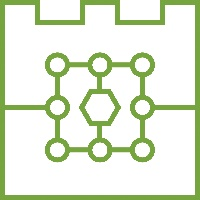
\includegraphics[width=2.31cm,height=2.31cm]{grafika/logo-wiim.jpg}};
    \node[anchor=north, text width=10.55cm, align=center] at ($(M)+(7.79cm,-0.25cm)$)
      {\fontsize{16pt}{21.2pt}\selectfont
       \textbf{Politechnika Krakowska\\im. Tadeusza Kościuszki}\\[10pt]
       Wydział Informatyki i Matematyki};
    \node[anchor=north, text width=11.1cm, align=center] at ($(M)+(8.29cm,-6.79cm)$)
      {\fontsize{14pt}{18.5pt}\selectfont\textbf{\autorpracy}\\[10pt]
       \fontsize{12pt}{15.9pt}\selectfont Numer albumu: \numeralbumu};
    \node[anchor=north, text width=13.38cm, align=center] at ($(M)+(8cm,-9.75cm)$)
      {\fontsize{16pt}{21.2pt}\selectfont\bfseries
       \pk@blokmin{1.98cm}{\tytulpl}%
       \pk@blokmin{1.85cm}{\tytulen}%
       \fontsize{14pt}{18.5pt}\selectfont
       Praca \rodzajpracy\\na kierunku \kierunek\par
       \vskip 10pt specjalność \specjalnosc\par};
    \node[anchor=north west, text width=8.6cm, align=left] at ($(M)+(7.12cm,-17.7cm)$)
      {\fontsize{12pt}{15.9pt}\selectfont\bfseries
       Praca wykonana pod kierunkiem:\\\promotor};
    \node[anchor=north, align=center] at ($(M)+(8cm,-24.11cm)$)
      {\fontsize{12pt}{15.9pt}\selectfont\bfseries \miejsce, \rokpracy};
  \end{tikzpicture}%
  \endgroup
  \clearpage}
\makeatother

\begin{document}

\stronatytulowa

\begin{singlespace}
  \tableofcontents
\end{singlespace}

\rozdzialnienumerowany{Wykaz ważniejszych oznaczeń i skrótów}

\begin{description}[style=sameline, leftmargin=2.8cm, labelwidth=2.5cm,
    labelsep=0.3cm, font=\normalfont]
  \item[DA] -- dostępność danych (ang.~\textit{Data Availability}),
  \item[DAS] -- próbkowanie dostępności danych (ang.~\textit{Data Availability Sampling}),
  \item[KZG] -- zobowiązanie wielomianowe Kate–Zaverucha–Goldberga (ang.~\textit{KZG polynomial commitment}),
  \item[L2] -- warstwa druga (ang.~\textit{Layer 2}),
  \item[NMT] -- drzewo Merkle'a z przestrzeniami nazw (ang.~\textit{Namespaced Merkle Tree}),
  \item[RS] -- kod Reeda–Solomona,
  \item[$k$] -- rozmiar boku macierzy danych oryginalnych,
  \item[$s$] -- liczba próbek pobieranych przez lekki węzeł.
\end{description}

\chapter{Wstęp}
\label{chap:wstep}

[Treść wstępu.] Problem dostępności danych w~systemach blockchain został
sformułowany m.in. w~pracach~\cite{AlBassam2018Fraud, ButerinDANote}, a~jego
formalny model przedstawiono w~\cite{HallAndersen2024Foundations}. Przykład
odwołania do kilku kolejnych pozycji: \cite{AlBassam2018Fraud,
  HallAndersen2024Foundations, ButerinDANote}.

\chapter{Cel i zakres pracy}
\label{chap:cel}

Celem pracy jest [\dots].

[Hipoteza badawcza.]

Zakres pracy obejmuje:
\begin{itemize}
  \item przegląd architektury modularnych systemów blockchain i~problemu
        dostępności danych (rozdz.~\ref{chap:modularne}),
  \item omówienie mechanizmu DAS i~jego implementacji (rozdz.~\ref{chap:das}),
  \item opracowanie metody oceny skuteczności DAS (rozdz.~\ref{chap:metoda}),
  \item projekt i~implementację środowiska eksperymentalnego
        (rozdz.~\ref{chap:implementacja}),
  \item badania eksperymentalne i~analizę wyników (rozdz.~\ref{chap:badania}).
\end{itemize}

\chapter{Modularne systemy blockchain i problem dostępności danych}
\label{chap:modularne}

[Krótkie wprowadzenie do rozdziału.]

\section{Architektura modularna}
\label{sec:architektura}

[Treść podrozdziału.] Przypisy dodatkowe (niebędące bibliografią) umieszcza się
u~dołu strony\footnote{Przykład przypisu dolnego.}.

\subsection{Warstwa dostępności danych}

[Treść punktu podrozdziału.]

\section{Atak polegający na ukrywaniu danych}

 [Treść podrozdziału.]

\chapter{Mechanizm Data Availability Sampling}
\label{chap:das}

[Krótkie wprowadzenie do rozdziału.]

\section{Kodowanie Reeda-Solomona w dwóch wymiarach}

Na rys.~\ref{fig:kwadrat} zaprezentowano schemat rozszerzenia macierzy danych
o~wymiarach $k \times k$ do macierzy $2k \times 2k$.

\begin{figure}[htbp]
  \begin{tikzpicture}[scale=1.25]
    \fill[gray!25] (0,2) rectangle (2,4);
    \fill[gray!8]  (2,2) rectangle (4,4);
    \fill[gray!8]  (0,0) rectangle (2,2);
    \fill[gray!8]  (2,0) rectangle (4,2);
    \draw[step=0.5, gray!60, very thin] (0,0) grid (4,4);
    \draw[thick] (0,0) rectangle (4,4);
    \draw[thick] (2,0) -- (2,4) (0,2) -- (4,2);
    \node at (1,3) {dane};
    \node[align=center, font=\fontsize{10pt}{12pt}\selectfont] at (3,3) {parzystość\\wierszy};
    \node[align=center, font=\fontsize{10pt}{12pt}\selectfont] at (1,1) {parzystość\\kolumn};
    \node[align=center, font=\fontsize{10pt}{12pt}\selectfont] at (3,1) {parzystość\\parzystości};
    \draw[{Latex}-{Latex}] (0,4.3) -- node[above] {$2k$} (4,4.3);
    \draw[{Latex}-{Latex}] (-0.3,2) -- node[left] {$k$} (-0.3,4);
  \end{tikzpicture}
  \caption{Rozszerzona macierz danych w~kodowaniu dwuwymiarowym (opracowanie własne na podstawie~\cite{AlBassam2018Fraud})}
  \label{fig:kwadrat}
\end{figure}

[Pierwszy akapit pod rysunkiem.]

\section{Implementacje: Celestia, PeerDAS, EigenDA}

 [Treść podrozdziału, np. odwołanie do specyfikacji~\cite{EIP7594}.]

\chapter{Metoda oceny skuteczności DAS}
\label{chap:metoda}

[Krótkie wprowadzenie do rozdziału.]

\section{Model analityczny}

Jeżeli producent bloku ukrywa ułamek $f$ fragmentów danych, a~lekki węzeł
pobiera $s$ niezależnych próbek ze zwracaniem, to prawdopodobieństwo, że
żadna z~próbek nie trafi w~ukryty fragment, wynosi
\begin{equation}
  P_{\mathrm{fail}} = (1 - f)^{s},
  \label{eq:pfail}
\end{equation}
gdzie: $f$ -- ułamek ukrytych fragmentów, $s$ -- liczba próbek.
Zależność~(\ref{eq:pfail}) umożliwia oszacowanie liczby próbek potrzebnej do
osiągnięcia zadanego poziomu bezpieczeństwa~\cite{Mitzenmacher2017}.

\section{Metryki}

W~tabeli~\ref{tab:metryki} zestawiono metryki wykorzystywane w~ocenie.

\begin{table}[htbp]
  \caption{Metryki oceny mechanizmu DAS}
  \label{tab:metryki}
  \begin{tabularx}{\linewidth}{|X|X|}
    \hline
    Bezpieczeństwo                & Skalowalność                         \\ \hline
    prawdopodobieństwo wykrycia   & transfer danych na węzeł             \\ \hline
    odsetek fałszywych akceptacji & czas próbkowania                     \\ \hline
    odsetek oszukanych węzłów     & koszt weryfikacji dowodów            \\ \hline
    skuteczność rekonstrukcji     & wpływ liczby węzłów i~rozmiaru bloku \\ \hline
  \end{tabularx}
\end{table}

[Pierwszy akapit pod tabelą.]

\chapter{Projekt i implementacja środowiska eksperymentalnego}
\label{chap:implementacja}

[Krótkie wprowadzenie do rozdziału.]

\section{Generator scenariuszy}

Na listingu~\ref{lst:scenariusz} przedstawiono przykładową konfigurację
scenariusza.

\begin{lstlisting}[caption={Przykładowa konfiguracja scenariusza}, label={lst:scenariusz}]
{
  "scenario": "withholding_2d",
  "k": 64,
  "samples_per_node": 16,
  "nodes": 1000,
  "seed": 42
}
\end{lstlisting}

\chapter{Badania eksperymentalne i analiza wyników}
\label{chap:badania}

[Krótkie wprowadzenie do rozdziału.]

\section{Walidacja symulatora}

 [Treść podrozdziału.]

\rozdzialnienumerowany{Podsumowanie}

[Treść podsumowania.]

\clearpage
\phantomsection
\addcontentsline{toc}{chapter}{\bibname}
\begin{singlespace}
  \bibliographystyle{pk-numeric}
  \bibliography{bibliografia}
\end{singlespace}

\spiswtresci{\listfigurename}{\listoffigures}
\spiswtresci{\listtablename}{\listoftables}
\spiswtresci{\lstlistlistingname}{\lstlistoflistings}

\appendix

\chapter{Konfiguracje eksperymentów}

 [Treść aneksu, np. pełne konfiguracje scenariuszy i~adres repozytorium.]

\end{document}
